\section{研究设计}
\label{sec:design}

价格数据。行情数据来自腾讯财经公开行情接口，逐只证券采集日频价格。
为保证总收益口径正确，本文对每只证券同时保留两套序列：不复权价格用于流动性排序、
涨跌停判定与成交价确定，其经济含义不随复权基准漂移；后复权价格用于计算含分红送转的
持有期总收益。后复权序列在任一日期之后仅相差一个常数复权因子，
相邻两日之比恰等于真实总收益率，不引入未来信息。实践中常见的前复权价格以当前为基准
向前调整，会随新的分红事件改变历史序列，在滚动回测中造成信息泄漏，本文不予采用。

样本范围。上海与深圳 A 股，2006 年 1 月至 2026 年 7 月，共 247 个月度形成期，
包含 868 只证券，月均进入股票池 438 只。股票池规模由 2006 年的 306 只增至 2025 年的
523 只（表 \ref{tab:universe}）。

\begin{table}[htbp]
\centering
\caption{股票池规模的年度分布}
\label{tab:universe}
\begin{threeparttable}
\small
\begin{tabular}{lrrrrrrrrrr}
\toprule
年份 & 2006 & 2008 & 2010 & 2012 & 2014 & 2016 & 2018 & 2020 & 2022 & 2025 \\
\midrule
月均股票池 & 306 & 386 & 437 & 442 & 429 & 413 & 428 & 455 & 482 & 523 \\
\bottomrule
\end{tabular}
\begin{tablenotes}[flushleft]\footnotesize
\item 注：股票池按本节的点时规则每月重新确定。样本整体覆盖 868 只证券、
247 个月度形成期，月均 438 只。
\end{tablenotes}
\end{threeparttable}
\end{table}

\begin{figure}[htbp]
\centering
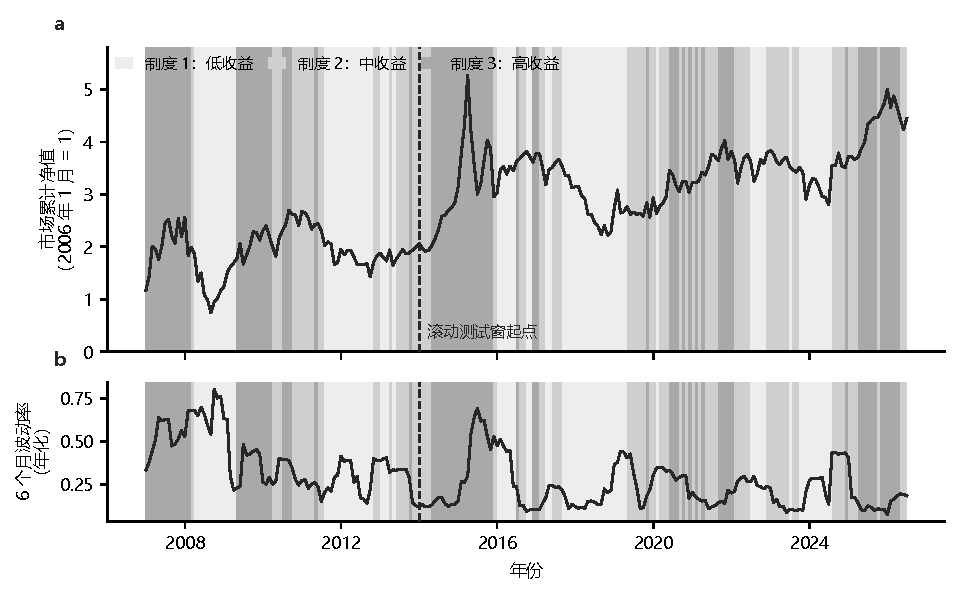
\includegraphics[width=\textwidth]{fig_regime.pdf}
\caption{样本期的市场环境与制度划分（2006--2026 年）}
\label{fig:regime}
\begin{minipage}{0.94\textwidth}\footnotesize
注：上图为市场累计净值（2006 年 1 月 = 1），底纹表示按 12 个月市场收益三分位
划分的制度状态；下图为 6 个月滚动波动率（年化）。竖虚线标出滚动测试窗起点。
状态划分与后文使用的制度变量一致，样本为沪深 A 股月度收益（247 个月）。
\end{minipage}
\end{figure}

点时股票池规则。每月形成日按四条规则筛选，条件只使用形成日及之前的信息：
当月至少有 5 个交易日（剔除长期停牌）、非 ST 类证券、上市满 6 个月、
成交额处于横截面 30\% 分位以上。四条规则分别剔除流动性中断、特殊处理、
新股与低流动性证券。

退市处理。证券列表包含已退市与已摘牌证券。有执行价但随后无行情的观测，
收益记为 $-1$，以控制幸存者偏差。本文区分两种情形：真实退市指有执行价但因数据中断
而没有退出价，收益记 $-1$；数据右边界指最后一个观测月及其前一月，
其退出价落在尚未观测到的下一个月，该整月从样本中剔除，以保证横截面在月份间可比。
样本中的真实退市观测为 8 个。公开行情接口对部分早期退市证券已不提供历史数据，
退市损失的覆盖因此偏低，结果相对乐观；由于本文的核心结论是门控优势不显著，
这一方向性偏差不改变主要判断（第 \ref{sec:robust} 节详述）。

执行采用严格点时规则：$t$ 月末收盘观测全部特征与市场状态，形成目标权重 $w_t$；
$t+1$ 月第一个交易日收盘按该日价格建仓；持有至 $t+2$ 月第一个交易日收盘换仓。
单期持有收益为后复权价之比。该规则比「月末收盘直接成交」保守，
不允许策略利用月末最后一个交易日的收盘价立即建仓，避免信号与成交价同时可观测的隐性前视。

换手按漂移后权重与目标权重之差的半 $L_1$ 范数计算，
交易成本为单边 $\kappa=10$ 个基点，从当期收益中扣除。
第 \ref{sec:marginal} 节与第 \ref{sec:robust} 节报告 $\kappa\in\{0,5,10,20,30,50\}$
基点的边际效应与敏感性。执行月首三个交易日触及涨停的证券标记为不可买入，
其权重按剩余可交易证券的比例再分配，使回测不依赖无法成交的价格；
涨跌停幅度按板块设定，科创板与创业板为 20\%，其余为 10\%。

本文的多智能体策略由五个专家智能体与一个门控智能体构成。
五个专家智能体为线性可解释信号（表 \ref{tab:expert-def}），门控智能体负责按状态分配权重。
打分方向由金融理论设定，不参与自由训练。该约束同时保证参数可识别：
若专家参数与门控参数自由联合训练，式 \eqref{eq:softmax-expert} 的 softmax 映射
具有平移不变性（$\theta$ 与 $\theta+c\bone$ 给出同一组合），
门控可通过缩放 $\tau_k$ 复制专家的任意强度变化，参数不可识别。

\begin{table}[htbp]
\centering
\caption{专家信号定义}
\label{tab:expert-def}
\begin{threeparttable}
\small
\begin{tabular}{lll}
\toprule
专家 & 打分 & 经济含义 \\
\midrule
动量 & $0.7\,\mathrm{mom}_{12-1}+0.3\,\mathrm{mom}_{12}$ & 中期价格趋势 \\
反转 & $-1.0\,\mathrm{mom}_{1}$ & 短期过度反应修正 \\
低波动 & $-1.0\,\mathrm{vol}_{60}$ & 低风险异象 \\
低换手 & $0.4\,\mathrm{mom}_{12-1}-0.6\,\mathrm{turnover}_{20}$ & 低流动性溢价 \\
低 beta & $0.3\,\mathrm{mom}_{12-1}-1.0\,\beta_{120}$ & 系统性风险规避 \\
\bottomrule
\end{tabular}
\begin{tablenotes}[flushleft]\footnotesize
\item 注：全部特征在每月横截面做 1\%--99\% 缩尾后标准化。
$\mathrm{mom}_{12-1}$ 为过去 12 个月剔除最近 1 个月的累计收益，
$\mathrm{mom}_{12}$ 为过去 12 个月累计收益，$\mathrm{mom}_{1}$ 为最近 1 个月收益；
$\mathrm{vol}_{60}$ 为 60 日收益标准差；$\mathrm{turnover}_{20}$ 为异常成交量
（20 日均量除以 250 日均量），因公开行情接口不提供换手率字段，以成交量口径替代；
$\beta_{120}$ 为 120 日滚动市场 beta。
\end{tablenotes}
\end{threeparttable}
\end{table}

打分经带温度参数 $\tau=0.6$ 的 softmax 映射为长仓满仓权重。
五个专家组合相对等权的平均半 $L_1$ 距离依次为：动量 0.431、反转 0.483、低波动 0.502、
低换手 0.336、低 beta 0.165，五个专家都产生了实质性不同于等权的持仓。
作为对照，梯度提升树策略的主动暴露仅为 0.005。

门控网络与训练目标。门控输入包含四组信息：市场制度变量（7 个）包括 3 个月与 12 个月市场收益、
6 个月波动率、6 个月趋势、1 年回撤、横截面离散度、上涨股票占比，
全部在训练窗内做扩展窗标准化；专家置信度为各专家截面打分的标准差；
专家风险为各专家组合的加权平均波动率；专家近期表现为指数加权历史收益
（衰减率 0.85），只使用当期之前的信息。门控为两层 tanh 网络（隐层 24 单元），
输出经 softmax 得到专家权重，组合自动满足长仓满仓约束。

训练目标为式 \eqref{eq:active-objective} 的主动收益型目标。信息比率项、CVaR 项
（5\% 尾部）、换手项与熵项的相对权重由验证窗在预先设定的 $3\times2$ 网格上选择，
测试窗不参与任何参数选择。门控网络的全部解析梯度经中心差分数值检验，
六种参数组合下的最大相对误差低于 $2\times10^{-6}$。该检验在实现过程中揭示了两类错误：
熵项与换手项缺失均值因子导致梯度按 $T$ 倍高估；标准差分母的数值稳定项经 $1/\sigma^3$
放大约 100 倍。两类错误均不导致程序报错，但会使训练结果无意义。

滚动样本外设计与推断。每个测试年份独立重估：训练窗为测试年前第 7 至第 2 年（5 年），
验证窗为测试年前 1 年，测试窗为测试当年。测试年份为 2014--2025 年，共 12 个年度窗口。
学习模型在每个窗口使用三个随机种子（7、19、42）重复，报告时先在年内对种子取平均，
再以年份为配对单位推断。相对基准的差异用循环区块自助法（块长 2 年，10\,000 次重抽样）
构造 95\% 区间，辅以 Wilcoxon 符号秩检验；对所有基准的多重比较采用 Holm 逐步校正；
模型整体排序差异用 Friedman 检验。随机种子用于度量优化不确定性，不作为额外的市场年份：
若把 3 个种子与 12 年当作 36 个独立观测，标准误将被低估约 $\sqrt{3}$ 倍。

互补性统计量由两个口径估计。第一个口径为月度横截面回归
\begin{equation}
r_{i,t+1}=a_t+\sum_{j=1}^J c_{j,t}\,\tilde x_{j,i,t}+\varepsilon_{i,t+1},
\label{eq:cs-regression}
\end{equation}
其中 $\tilde x_{j,i,t}$ 为第 $j$ 个特征在当月横截面标准化后的取值。
按制度归并回归系数 $c_{j,t}$ 得到 $\hat\Gamma^{\text{IC}}$。
第二个口径基于专家组合收益在制度内的均值与标准差，记为 $\hat\Gamma^{(1)}$
与 $\hat\Gamma^{(2)}$。

噪声底线的自校准用循环区块自助法：把制度标签在时间上做区块重抽样，
破坏制度与收益的对应关系，重新计算统计量，取分布的 95\% 分位数作为 $\Theta$。
该分布在无真实互补性时仍会因抽样噪声产生正值，其高分位数即「不可区分于噪声」的临界水平。
该设计不依赖式 \eqref{eq:theta-def} 中对 $\sigma_b$ 与 $\rho_k$ 的参数假设。
两个技术要点：$K$ 个专家的收益在横截面上高度相关，重抽样按整期联合抽取；
区块长度需覆盖制度内部的序列相关，本文取 12 个月，其敏感性见第 \ref{sec:robust} 节。
此外，按专家收益的平均两两相关估计有效独立专家数
$\hat K_{\text{eff}}=K/[1+(K-1)\bar\rho]$，并据此对自助分布的离散度做保守校正。

Oracle 门控与安慰剂检验。Oracle 门控按
$g^{\text{oracle}}_{k,s}\propto\exp(\eta\bar a_k^\top\hat\bmu_s)$ 构造，
其中 $\hat\bmu_s$ 为训练窗内制度 $s$ 的资产平均持有期收益。它使用制度内真实条件期望收益，
不可实现，仅用于度量一阶互补性的可利用上界。安慰剂检验保持门控输入与专家权重不变，
把资产收益矩阵在时间维度做循环区块置换后重新训练门控，重复 200 次；
同时计算制度间的变异系数 $\mathrm{CV}^{(1)}$（条件均值）与 $\mathrm{CV}^{(2)}$
（条件波动），并用区块置换构造零分布。
